% Options for packages loaded elsewhere
\PassOptionsToPackage{unicode}{hyperref}
\PassOptionsToPackage{hyphens}{url}
\PassOptionsToPackage{dvipsnames,svgnames,x11names}{xcolor}
%
\documentclass[
  letterpaper,
  DIV=11,
  numbers=noendperiod]{scrreprt}

\usepackage{amsmath,amssymb}
\usepackage{iftex}
\ifPDFTeX
  \usepackage[T1]{fontenc}
  \usepackage[utf8]{inputenc}
  \usepackage{textcomp} % provide euro and other symbols
\else % if luatex or xetex
  \usepackage{unicode-math}
  \defaultfontfeatures{Scale=MatchLowercase}
  \defaultfontfeatures[\rmfamily]{Ligatures=TeX,Scale=1}
\fi
\usepackage{lmodern}
\ifPDFTeX\else  
    % xetex/luatex font selection
\fi
% Use upquote if available, for straight quotes in verbatim environments
\IfFileExists{upquote.sty}{\usepackage{upquote}}{}
\IfFileExists{microtype.sty}{% use microtype if available
  \usepackage[]{microtype}
  \UseMicrotypeSet[protrusion]{basicmath} % disable protrusion for tt fonts
}{}
\makeatletter
\@ifundefined{KOMAClassName}{% if non-KOMA class
  \IfFileExists{parskip.sty}{%
    \usepackage{parskip}
  }{% else
    \setlength{\parindent}{0pt}
    \setlength{\parskip}{6pt plus 2pt minus 1pt}}
}{% if KOMA class
  \KOMAoptions{parskip=half}}
\makeatother
\usepackage{xcolor}
\setlength{\emergencystretch}{3em} % prevent overfull lines
\setcounter{secnumdepth}{5}
% Make \paragraph and \subparagraph free-standing
\ifx\paragraph\undefined\else
  \let\oldparagraph\paragraph
  \renewcommand{\paragraph}[1]{\oldparagraph{#1}\mbox{}}
\fi
\ifx\subparagraph\undefined\else
  \let\oldsubparagraph\subparagraph
  \renewcommand{\subparagraph}[1]{\oldsubparagraph{#1}\mbox{}}
\fi


\providecommand{\tightlist}{%
  \setlength{\itemsep}{0pt}\setlength{\parskip}{0pt}}\usepackage{longtable,booktabs,array}
\usepackage{calc} % for calculating minipage widths
% Correct order of tables after \paragraph or \subparagraph
\usepackage{etoolbox}
\makeatletter
\patchcmd\longtable{\par}{\if@noskipsec\mbox{}\fi\par}{}{}
\makeatother
% Allow footnotes in longtable head/foot
\IfFileExists{footnotehyper.sty}{\usepackage{footnotehyper}}{\usepackage{footnote}}
\makesavenoteenv{longtable}
\usepackage{graphicx}
\makeatletter
\def\maxwidth{\ifdim\Gin@nat@width>\linewidth\linewidth\else\Gin@nat@width\fi}
\def\maxheight{\ifdim\Gin@nat@height>\textheight\textheight\else\Gin@nat@height\fi}
\makeatother
% Scale images if necessary, so that they will not overflow the page
% margins by default, and it is still possible to overwrite the defaults
% using explicit options in \includegraphics[width, height, ...]{}
\setkeys{Gin}{width=\maxwidth,height=\maxheight,keepaspectratio}
% Set default figure placement to htbp
\makeatletter
\def\fps@figure{htbp}
\makeatother
\newlength{\cslhangindent}
\setlength{\cslhangindent}{1.5em}
\newlength{\csllabelwidth}
\setlength{\csllabelwidth}{3em}
\newlength{\cslentryspacingunit} % times entry-spacing
\setlength{\cslentryspacingunit}{\parskip}
\newenvironment{CSLReferences}[2] % #1 hanging-ident, #2 entry spacing
 {% don't indent paragraphs
  \setlength{\parindent}{0pt}
  % turn on hanging indent if param 1 is 1
  \ifodd #1
  \let\oldpar\par
  \def\par{\hangindent=\cslhangindent\oldpar}
  \fi
  % set entry spacing
  \setlength{\parskip}{#2\cslentryspacingunit}
 }%
 {}
\usepackage{calc}
\newcommand{\CSLBlock}[1]{#1\hfill\break}
\newcommand{\CSLLeftMargin}[1]{\parbox[t]{\csllabelwidth}{#1}}
\newcommand{\CSLRightInline}[1]{\parbox[t]{\linewidth - \csllabelwidth}{#1}\break}
\newcommand{\CSLIndent}[1]{\hspace{\cslhangindent}#1}

\KOMAoption{captions}{tableheading}
\usepackage{fontspec}
\setmainfont{Arial}
\setsansfont{Arial}
\usepackage{anyfontsize}
\fontsize{11}{16}\selectfont
\usepackage{booktabs}
\usepackage{graphicx}
\usepackage[nottoc]{tocbibind}
\usepackage{natbib}
\PassOptionsToPackage{table}{xcolor}
\usepackage{xcolor}
\renewcommand{\bibsection}{}
\usepackage[a4paper, top=2.5cm, bottom=3cm, left=2.5cm, right=2.5cm]{geometry}
\usepackage{tocloft}
\setlength{\cftbeforetoctitleskip}{0pt}
\renewcommand{\cftsecleader}{\cftdotfill{\cftdotsep}}
\usepackage{scrhack}
\usepackage{etoolbox}
\makeatletter
\patchcmd{\chapter}{\if@openright\cleardoublepage\else\clearpage\fi}{}{}{}
\makeatother
\RedeclareSectionCommand[ beforeskip=12pt plus 1pt minus 1pt, afterskip=6pt plus 1pt minus 1pt, font=\fontsize{16pt}{20pt}\bfseries\sffamily, ]{chapter}
\RedeclareSectionCommand[ beforeskip=10pt plus 1pt minus 1pt, afterskip=5pt plus 1pt minus 1pt, font=\fontsize{14pt}{18pt}\bfseries\sffamily, ]{section}
\RedeclareSectionCommand[ beforeskip=8pt plus 1pt minus 1pt, afterskip=4pt plus 1pt minus 1pt, font=\fontsize{12pt}{16pt}\bfseries\sffamily, ]{subsection}
\RedeclareSectionCommand[ beforeskip=6pt plus 1pt minus 1pt, afterskip=3pt plus 1pt minus 1pt, font=\fontsize{10pt}{14pt}\bfseries\sffamily, ]{subsubsection}
\RedeclareSectionCommand[ beforeskip=4pt plus 1pt minus 1pt, afterskip=2pt plus 1pt minus 1pt, font=\fontsize{10pt}{12pt}\bfseries\sffamily, ]{paragraph}
\RedeclareSectionCommand[ beforeskip=2pt plus 1pt minus 1pt, afterskip=1pt plus 1pt minus 1pt, font=\fontsize{8pt}{10pt}\bfseries\sffamily, ]{subparagraph}
\makeatletter
\makeatother
\makeatletter
\@ifpackageloaded{bookmark}{}{\usepackage{bookmark}}
\makeatother
\makeatletter
\@ifpackageloaded{caption}{}{\usepackage{caption}}
\AtBeginDocument{%
\ifdefined\contentsname
  \renewcommand*\contentsname{Table of contents}
\else
  \newcommand\contentsname{Table of contents}
\fi
\ifdefined\listfigurename
  \renewcommand*\listfigurename{List of Figures}
\else
  \newcommand\listfigurename{List of Figures}
\fi
\ifdefined\listtablename
  \renewcommand*\listtablename{List of Tables}
\else
  \newcommand\listtablename{List of Tables}
\fi
\ifdefined\figurename
  \renewcommand*\figurename{Figure}
\else
  \newcommand\figurename{Figure}
\fi
\ifdefined\tablename
  \renewcommand*\tablename{Table}
\else
  \newcommand\tablename{Table}
\fi
}
\@ifpackageloaded{float}{}{\usepackage{float}}
\floatstyle{ruled}
\@ifundefined{c@chapter}{\newfloat{codelisting}{h}{lop}}{\newfloat{codelisting}{h}{lop}[chapter]}
\floatname{codelisting}{Listing}
\newcommand*\listoflistings{\listof{codelisting}{List of Listings}}
\makeatother
\makeatletter
\@ifpackageloaded{caption}{}{\usepackage{caption}}
\@ifpackageloaded{subcaption}{}{\usepackage{subcaption}}
\makeatother
\makeatletter
\@ifpackageloaded{tcolorbox}{}{\usepackage[skins,breakable]{tcolorbox}}
\makeatother
\makeatletter
\@ifundefined{shadecolor}{\definecolor{shadecolor}{rgb}{.97, .97, .97}}
\makeatother
\makeatletter
\makeatother
\makeatletter
\makeatother
\ifLuaTeX
  \usepackage{selnolig}  % disable illegal ligatures
\fi
\IfFileExists{bookmark.sty}{\usepackage{bookmark}}{\usepackage{hyperref}}
\IfFileExists{xurl.sty}{\usepackage{xurl}}{} % add URL line breaks if available
\urlstyle{same} % disable monospaced font for URLs
\hypersetup{
  pdfauthor={Robin Pfaff},
  colorlinks=true,
  linkcolor={black},
  filecolor={Maroon},
  citecolor={Blue},
  urlcolor={Blue},
  pdfcreator={LaTeX via pandoc}}

\author{Robin Pfaff}
\date{2023-06-27}

\begin{document}
\begin{titlepage}
    \centering
    {\fontsize{12}{10}\selectfont ZURICH UNIVERSITY OF APPLIED SCIENCES\par}
    {\fontsize{12}{10}\selectfont SCHOOL OF LIFE SCIENCES AND FACILITY MANAGEMENT\par}
    {\fontsize{12}{10}\selectfont INSTITUTE OF NATURAL RESOURCE SCIENCES\par}
    \vspace{6cm}
    {\fontsize{14}{16}\bfseries Quantification of deforestation on Borneo in the last 20 years based on open source geodata\par}
    {\fontsize{12}{14}\bfseries Bachelor Thesis\par}
    {\fontsize{12}{14}\selectfont HS23\par}
    \vspace{2cm}
    {\fontsize{12}{14}\bfseries by\par}
    {\fontsize{12}{14}\bfseries Robin Pfaff\par}
    {\fontsize{12}{14}\selectfont BSc Environmental engineering\par}
    \vspace{2cm}
    {\fontsize{12}{14}\selectfont Submission date: 28.10.2023\par}

    \vfill
    \begin{flushleft}
        1\textsuperscript{st} supervisor:\\
        Ochsner, Pascal\\
        2\textsuperscript{nd} supervisor:\\
        Ratnaweera, Nils\\
        ZHAW IUNR Research Group for Geoinformatics
    \end{flushleft}
\end{titlepage}

\clearpage
\pagenumbering{arabic}
\setcounter{page}{1}

\thispagestyle{empty}
\vspace*{\fill}

\noindent{\Large\textbf{Imprint}}

\vspace{0.5cm}

\noindent\textbf{Institute}\\
Institute of Natural Resource Sciences

\noindent\textbf{Form of citation}\\
APA 7th edition

\noindent\textbf{Keywords}\\
deforestation, spatiotemporal analysis, open source data, Boreno

\ifdefined\Shaded\renewenvironment{Shaded}{\begin{tcolorbox}[borderline west={3pt}{0pt}{shadecolor}, interior hidden, boxrule=0pt, enhanced, frame hidden, sharp corners, breakable]}{\end{tcolorbox}}\fi

\bookmarksetup{startatroot}

\hypertarget{abstract}{%
\chapter*{Abstract}\label{abstract}}

\markboth{Abstract}{Abstract}

\newpage
\tableofcontents

\bookmarksetup{startatroot}

\hypertarget{sec-introduction}{%
\chapter{Introduction}\label{sec-introduction}}

Borneo, the third largest island in the world, is home to large tropical
forests and peatlands. They have a vital ecological and climatic role on
a global scale and are of great socioeconomic value on a national and
regional level
(\protect\hyperlink{ref-harrisonTropicalForestPeatland2020}{Harrison et
al., 2020}). With an estimated 10,000 to 15,000 species of flowering
plants, 37 endemic bird and 44 endemic mammal species
(\protect\hyperlink{ref-mackinnonEcologyKalimantan1997}{MacKinnon et
al., 1997}), Borneo is part of the Sundaland biodiversity hotspot
(\protect\hyperlink{ref-myersBiodiversityHotspotsConservation2000}{Myers
et al., 2000}). However, this vast flora and fauna is threatened by land
use change, climate change and fire with the IUCN listing 415 species as
threatened
(\protect\hyperlink{ref-harrisonTropicalForestPeatland2020}{Harrison et
al., 2020}). Among them is the humans closest relative, the critically
endangered borneo orangutan {[}\emph{Pongo pygmaeus}; IUCN
(\protect\hyperlink{ref-iucnPongoPygmaeusAncrenaz2016}{2016}){]}. In
addition to biodiversity loss, these factors also have profound
consequences at the regional and global levels. Among them are
restrained water quality and quantity regulation services and greenhouse
gases (GHGs
\protect\hyperlink{ref-foleySolutionsCultivatedPlanet2011}{Foley et al.,
2011}). Because of these far-reaching consequences, measures to halt,
protect, or even reverse tropical deforestation have received increased
attention. This, for example, through incorporating regulatory
standards, corporate voluntary sustainability commitments, protected
area networks, economic incentives, and demand-side interventions
(\protect\hyperlink{ref-austinWhatCausesDeforestation2019}{Austin et
al., 2019}).

Vegetable oil producing crops such as canola, soybean, sunflower, and
oil palm occupy \textasciitilde7.5\%~of the world's agricultural land
with a total annual production of 217 Mt (2020 - 2022
\protect\hyperlink{ref-oecdOECDFAOAgriculturalOutlook2023}{OECD, 2023}).
This demand is expected to increase to 310 Mt by mid-century
(\protect\hyperlink{ref-byerleeTropicalOilCrop2016}{Byerlee et al.,
2016}), due to the increasing world population and as a renewable
resource for biofuel
(\protect\hyperlink{ref-abdulmajidSustainablePalmOil2021}{Abdul Majid et
al., 2021}). With a share of approximately one-third, palm oil is the
most widely used vegetable oil
(\protect\hyperlink{ref-kamyabElaeisGuineensis2022}{Kamyab, 2022};
\protect\hyperlink{ref-oecdOECDFAOAgriculturalOutlook2023}{OECD, 2023}).
The island of Borneo, which is shared between the two largest palm oil
producers in the world - Malaysia and Indonesia produce 85\% of the
world's palm oil - is a cultivation hotspot due to its tropical climate
and high rainfalls
(\protect\hyperlink{ref-kamyabElaeisGuineensis2022}{Kamyab, 2022}).

Although many recent global datasets provide the basis for analyzing the
key drivers of deforestation, the most recent study examining this for
Borneo was conducted a decade ago
(\protect\hyperlink{ref-gaveauFourDecadesForest2014}{Gaveau et al.,
2014}). Considering the global importance of this region, this paper
aims to fill this gap.

Building on open source geodata, this thesis investigates deforestation
and its drivers. The spatial extent is the island of Borneo, and its
temporal scope spans the past two decades. More precise, the following
questions are addressed: (i) what is the yearly extent of deforestation,
(ii) which influence did the introduction of the Roundtable for
Sustainable Palm Oil (RSPO) have on deforestation rates, (iii) how much
existing cropland was converted into oil palm plantations and (iv) how
does proximity to infrastructure impact deforestation rates? Annex ii
provides a list of the in-depth questions that help to answer these
guiding questions.

\begin{figure}[H]

{\centering 
\includegraphics[width=3.92in,height=1.4in]{text/03_introduction_files/figure-latex/mermaid-figure-1.png}

}

\end{figure}

Please see Figure @ref(fig:your-label) for the state diagram.

\bookmarksetup{startatroot}

\hypertarget{literature-review}{%
\chapter{Literature review}\label{literature-review}}

\hypertarget{deforestation}{%
\section{Deforestation}\label{deforestation}}

\hypertarget{infrastructure}{%
\section{Infrastructure}\label{infrastructure}}

\hypertarget{state-of-the-art-analysis}{%
\section{State of the art analysis}\label{state-of-the-art-analysis}}

\hypertarget{oil-palm-elaeis-guineensis-kamyabelaeisguineensis2022}{%
\section{\texorpdfstring{Oil palm \emph{(Elaeis guineensis)}
(\protect\hyperlink{ref-kamyabElaeisGuineensis2022}{Kamyab,
2022})}{Oil palm (Elaeis guineensis) (Kamyab, 2022)}}\label{oil-palm-elaeis-guineensis-kamyabelaeisguineensis2022}}

Originating from West Africa, the oil palm \emph{(Elaeis guineensis)} is
the most efficient and important oil-producing crop worldwide. It has
the highest yield in tropical climates with high rainfall, hence it is
successfully cultivated in Malaysia and Indonesia. These two countries
produce 85\% of the world's palm oil. Between 10 and 35 tons of fresh
fruit bunch (FFB) are harvested on one hectare. Oil extraction rates
(OER) have stagnated between 19 - 21\% over the past 40 years
(\protect\hyperlink{ref-changEconomicPerspectiveOil2003}{Chang et al.,
2003}; \protect\hyperlink{ref-chewImprovingSustainabilityPalm2021}{Chew
et al., 2021}). While the massive expansion of production capacities is
associated with economic growth and rapid development, the ecological
impact of giant oil palm monocultures and the environmental pollution
caused by large quantities of by-products during oil extraction pose
major problems. Palm oil is used in a

\hypertarget{rspo-abdulmajidsustainablepalmoil2021}{%
\section{\texorpdfstring{RSPO
(\protect\hyperlink{ref-abdulmajidSustainablePalmOil2021}{Abdul Majid et
al.,
2021})}{RSPO (Abdul Majid et al., 2021)}}\label{rspo-abdulmajidsustainablepalmoil2021}}

(Chapman et al.
(\protect\hyperlink{ref-chapmanCompoundingImpactDeforestation2020}{2020});
Descals et al.
(\protect\hyperlink{ref-descalsHighresolutionGlobalMap2021}{2021})).

\bookmarksetup{startatroot}

\hypertarget{sec-method}{%
\chapter{Method}\label{sec-method}}

\hypertarget{data-acquisition-and-selection}{%
\section{Data acquisition and
selection}\label{data-acquisition-and-selection}}

Initially, databases such as Web of Knowledge or Google Scholar were
searched for GIS and remote sensing studies covering Borneo, Southeast
Asia or even a global extent. QGIS (Version 3.30) was used for initial
data exploration. This led to the manual selection of data shown in
Figure~\ref{fig-data_overview} for further analysis. Hereafter, the
datasets are referred to by the names specified in the Content column.
The research area included the landmass of Borneo, explicitly excluding
the smaller surrounding islands. This delineation was obtained through
the OSMnx python package, which accesses the Open Street Maps (OSM)
database
(\protect\hyperlink{ref-boeingOSMnxPythonPackage2017}{\textbf{boeingOSMnxPythonPackage2017?}}).

\begin{figure}

{\centering 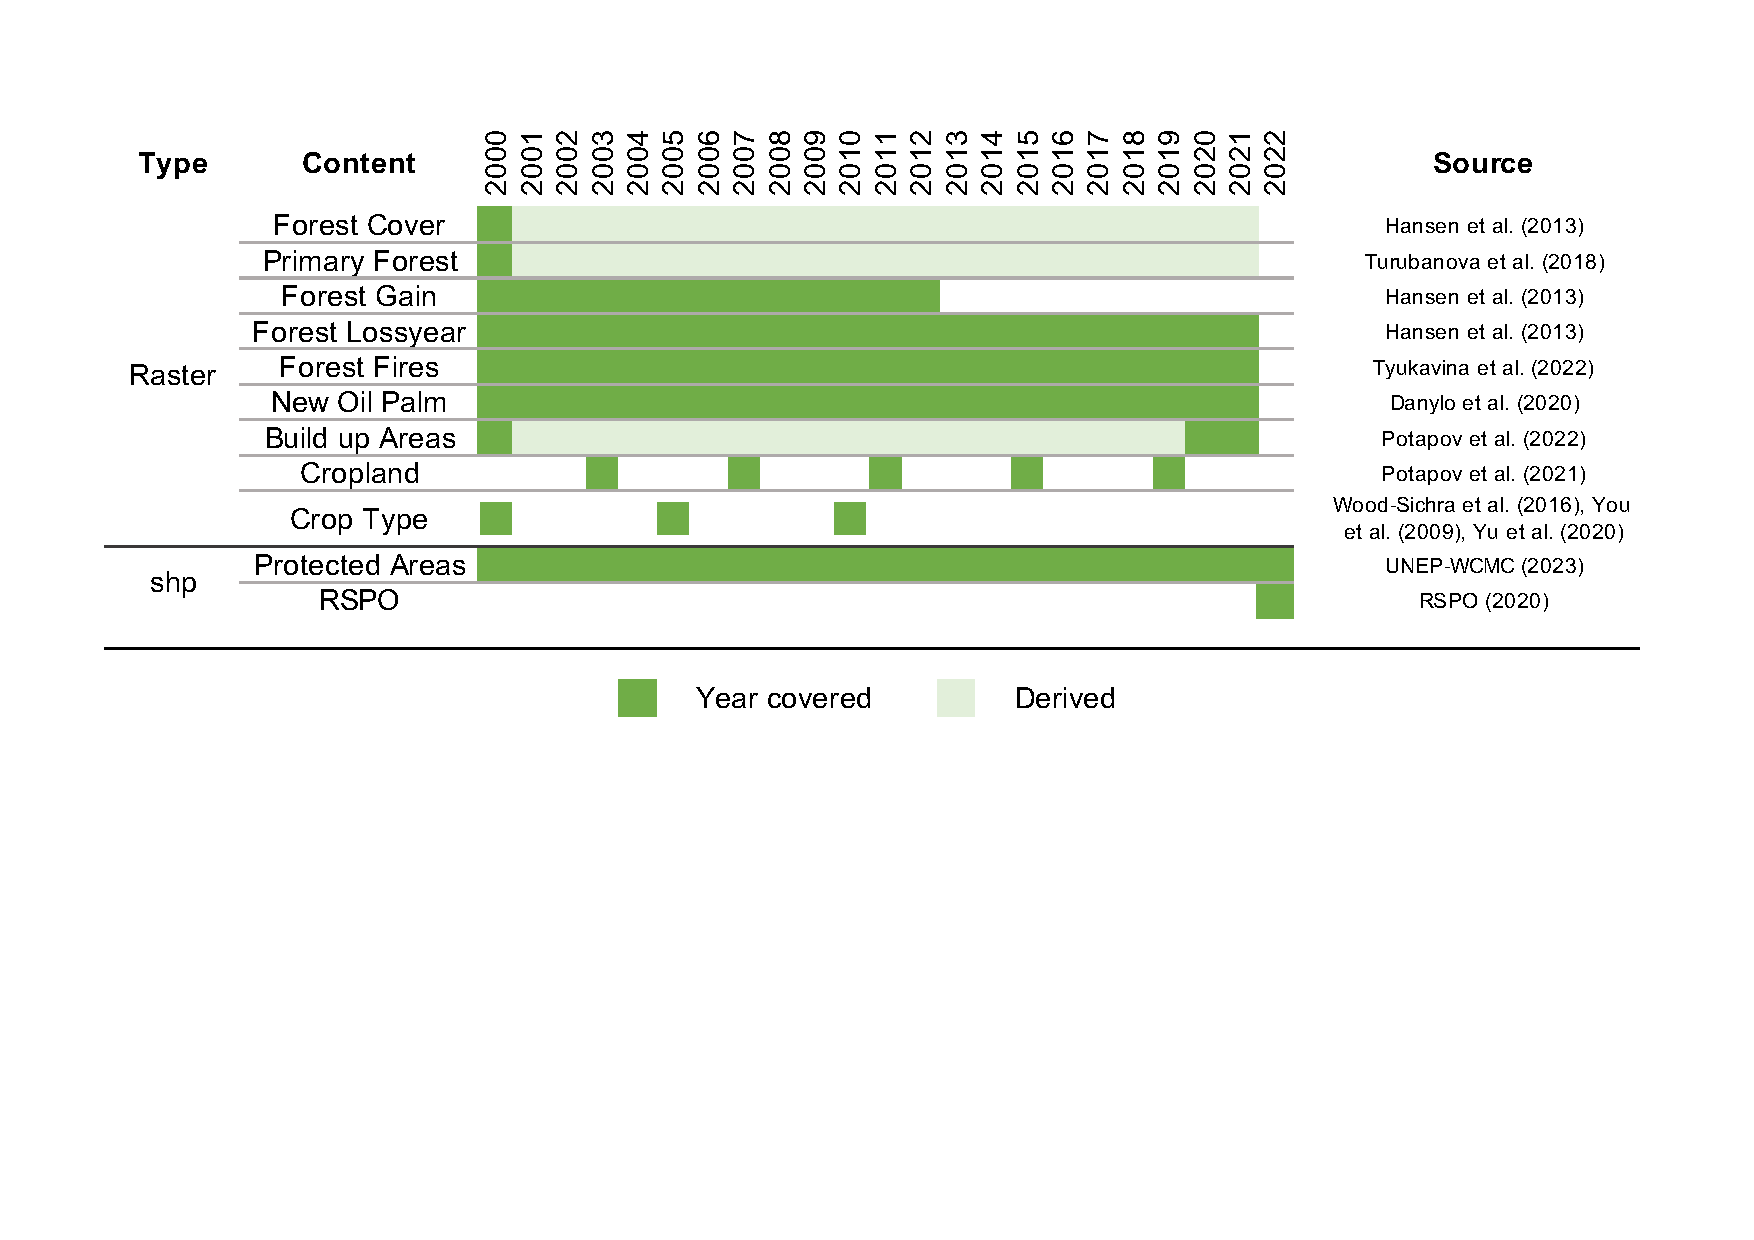
\includegraphics{text/05_method_files/data_overview.pdf}

}

\caption{\label{fig-data_overview}Example Picture 2}

\end{figure}

\hypertarget{data-preparation}{%
\section{Data preparation}\label{data-preparation}}

All datasets, which existed in several segments, were merged to cover at
least the extent of Borneo.

\begin{figure}

{\centering 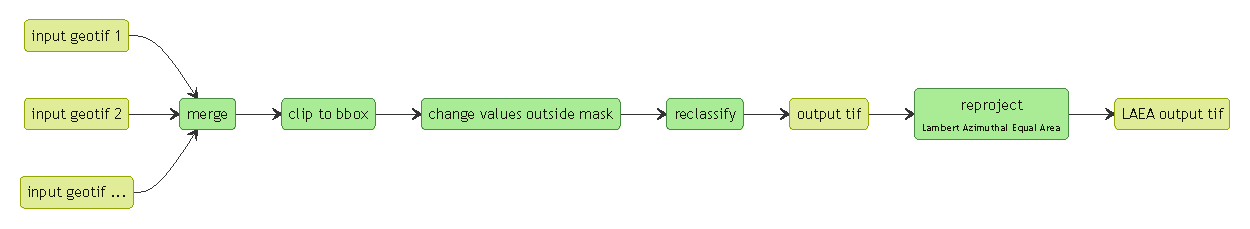
\includegraphics{text/../mermaid/raster_preparation.pdf}

}

\caption{\label{fig-mermaid}Flowchart}

\end{figure}

\hypertarget{data-processing}{%
\section{Data processing}\label{data-processing}}

For further analysis, a value of \textgreater50\% tree cover was
considered as forest
(\protect\hyperlink{ref-hansenHighResolutionGlobalMaps2013}{Hansen et
al., 2013}).

Aggregated plants and perennial woody plants such as coconut and oil
palm were manually removed from subsequent analysis due to the cropland
definition in the used dataset
(\protect\hyperlink{ref-potapovGlobalMapsCropland2021}{Potapov et al.,
2021}), as well as crops with total physical harvest area lower than
10000 ha within the project extent in any of the three datasets.

Please see Figure~\ref{fig-data_overview} for the table.

Figure~\ref{fig-mermaid}

\begin{longtable}[]{@{}llrc@{}}
\caption{Demonstration of pipe table syntax 1}\tabularnewline
\toprule\noalign{}
Default & Left & Right & Center \\
\midrule\noalign{}
\endfirsthead
\toprule\noalign{}
Default & Left & Right & Center \\
\midrule\noalign{}
\endhead
\bottomrule\noalign{}
\endlastfoot
12 & 12 & 12 & 12 \\
123 & 123 & 123 & 123 \\
1 & 1 & 1 & Hansen et al.
(\protect\hyperlink{ref-hansenHighResolutionGlobalMaps2013}{2013}) \\
\end{longtable}

\hypertarget{data-collection}{%
\section{Data Collection}\label{data-collection}}

\hypertarget{data-source}{%
\subsection{Data Source}\label{data-source}}

\bookmarksetup{startatroot}

\hypertarget{results}{%
\chapter{Results}\label{results}}

\hypertarget{questions}{%
\subsubsection{Questions}\label{questions}}

\hypertarget{general-forest-loss}{%
\subsubsection{General Forest loss}\label{general-forest-loss}}

\begin{enumerate}
\def\labelenumi{\arabic{enumi}.}
\tightlist
\item
  How much forest area was lost yearly and in total?
\item
  How much forest area was lost due to forest fires yearly and in total?
\item
  How much new build up areas was created on forest loss areas (2020
  compared to 2000)?
\item
  How much new build up areas was created on forest-fire loss areas
  (2020 compared to 2000)?
\item
  How much forest gain (area) occured on forest fire areas (2001 -
  2012)?
\item
  How much forest was lost in protected areas yearly? --\textgreater{}
  carry out all of them with primary forests as well
\end{enumerate}

\hypertarget{oil-palm-related}{%
\subsubsection{Oil Palm related}\label{oil-palm-related}}

\begin{enumerate}
\def\labelenumi{\arabic{enumi}.}
\tightlist
\item
  How much new oil palm plantation area occured yearly on forest fire
  areas?
\item
  How much new oil palm plantation area occured yearly on non-forest
  deforested areas?
\item
  How much new oil palm plantation area occured yearly on deforested
  areas?
\item
  How much new oil palm plantation area occured in protected ares?
\item
  How much new oil palm plantation areo occured on non-forest area?
  (compared to year 2000 forest cover)
\item
  How much new oil palm plantation area occured on previos cropland (and
  other way around)?
\item
  How much forest area was ganied on previous oil palm plantation area
  yearly (2000 - 2012)?
\item
  How much area was used for other crops prior to oil palm plantation,
  and which?
\item
  How much area was used for oil palm plantation prior to other crops,
  and which?
\end{enumerate}

\hypertarget{build-up-areas}{%
\subsubsection{Build up areas}\label{build-up-areas}}

\begin{enumerate}
\def\labelenumi{\arabic{enumi}.}
\tightlist
\item
  How much new build up area occured in forest covered area (2020
  compared to 2000)?
\item
  How much new build up area occured in non-forest covered area (2020
  compared to 2000)?
\item
  How much new build up area occured in forest fire area (2020 compared
  to 2000)?
\item
  How much new oil palm plantation area occured within 1, 2, 5, 10, and
  20 km of newly buld up areas?
\item
  How much forest area was lost to forest fires within 1, 2, 5, 10, and
  20 km of newly buld up areas?
\item
  How much forest area was lost to non-forest fires deforested areas
  within 1, 2, 5, 10, and 20 km of newly buld up areas?
\item
  How much forest area was lost to cropland areas within 1, 2, 5, 10,
  and 20 km of newly buld up areas?
\end{enumerate}

\hypertarget{rspo}{%
\subsubsection{RSPO}\label{rspo}}

???

For more information, refer to the literature review (Chapman et al.
(\protect\hyperlink{ref-chapmanCompoundingImpactDeforestation2020}{2020});
Descals et al.
(\protect\hyperlink{ref-descalsHighresolutionGlobalMap2021}{2021})).

\bookmarksetup{startatroot}

\hypertarget{discussion}{%
\chapter{Discussion}\label{discussion}}

However, the data showing forest gain in the span of 2001 - 2012 is
inaccurate. Analysis showed that 32\% of the alleged forest gain
represents newly established palm oil plantations. Thus, all new palm
oil cultivation areas established between 2001 and 2012 have been
removed from the forest gain dataset.

\hypertarget{data-selection}{%
\section{Data selection}\label{data-selection}}

\hypertarget{crop-harvest-area}{%
\subsection{Crop harvest area}\label{crop-harvest-area}}

Existing mapping of cropland all take a similar approach. They
disaggregate national and subnational statistics and estimate their
allocation to low-resolution grid cells of 5 arcminutes (Wood-Sichra et
al.
(\protect\hyperlink{ref-wood-sichraSpatialProductionAllocation2016}{2016});
You et al.
(\protect\hyperlink{ref-youGeneratingPlausibleCrop2009}{2009}); Yu et
al. (\protect\hyperlink{ref-yuCultivatedPlanet20102020}{2020}); Grogan
et al. (\protect\hyperlink{ref-groganGlobalGriddedCrop2022}{2022})).
Among them, the Spatial Production Allocation Model (SPAM) takes the
most factors into account rendering it the most comprehensive data. (You
\& Sun (\protect\hyperlink{ref-youMappingGlobalCropping2022}{2022}))
Additionally, the dataset family currently contains data for the years
2000, 2005 and 2010, which makes it the most suited choice for the
present work (Wood-Sichra et al.
(\protect\hyperlink{ref-wood-sichraSpatialProductionAllocation2016}{2016});
You et al.
(\protect\hyperlink{ref-youGeneratingPlausibleCrop2009}{2009}); Yu et
al. (\protect\hyperlink{ref-yuCultivatedPlanet20102020}{2020})).
However, due to improvements in the method of creating the datasets, the
more recent ones are a more accurate representation of the physical
harvest area and are more finely broken down into distinct crops.
(Wood-Sichra et al.
(\protect\hyperlink{ref-wood-sichraSpatialProductionAllocation2016}{2016});
Yu et al. (\protect\hyperlink{ref-yuCultivatedPlanet20102020}{2020})).
This is why coconut is missing in the year 2000 even though it was an
important crop for both Indonesia and Malaysia at that time
(\emph{{FAOSTAT}} (\protect\hyperlink{ref-FAOSTAT}{n.d.})).

Although a more recent dataset called Global Agro-ecological Zones (GAEZ
v4.0) was available for harvested crops in 2015, no analysis was
conducted with it because the data lacked the necessary quality and
therefore could not be compared to the SPAM datasets. Just like the SPAM
dataset, FAO statistics complemented with national data on FAO gaps,
were used to calculate crop yield in a 5 arcminute resolution grid.
However, the pixel values in the GAEZ 2015 dataset are based upon the
GAEZ 2010 (GAEZ v3.0) dataset, whose download portal does not work
anymore (FAO/IIASA
(\protect\hyperlink{ref-faoux2fiiasaGlobalAgroecologicalZones2010}{2010})).
It was calculated by multiplying the year GAEZ 2010 pixel value by the
countries' change in the given crop over the last 5 years. As a result,
any spatial displacement in the harvest area of a given crop to another
region is incorrectly mapped rendering the intended analysis inadequate.

Another available dataset for 2000 was neglected because the SPAM
datasets were all created using the same method, which reduces
inconsistency when comparing spatiotemporal differences. In addition,
only the harvested area was available in the alternative dataset. This
means that areas that were harvested several times per year were also
counted multiple times, biasing the total physically cultivated area.

Nevertheless, SPAM data is also subject to non-negligible drawbacks,
since \#\#\# !!!NOCH ERGÄNZEN!!! \#\#\# (Joglekar et al.
(\protect\hyperlink{ref-joglekarPixelatingCropProduction2019}{2019})).

\hypertarget{processing}{%
\section{Processing}\label{processing}}

As indicated before, merging data from different sources is challenging.
This is especially true for the croplands in higher resolution
(\textasciitilde30 m) with the physical harvest area for the individual
crops in lower resolution (5 arcminutes). Especially because the two
datasets were created with fundamentally different methods. While the
dataset of the cultivated areas was created by analysis of satellite
data time-series and showing their precise extent (Potapov et al.
(\protect\hyperlink{ref-potapovGlobalMapsCropland2021}{2021})), the
physical harvested area maps of the different crops were compiled by a
complex model based on statistics and estimates (Wood-Sichra et al.
(\protect\hyperlink{ref-wood-sichraSpatialProductionAllocation2016}{2016});
You et al.
(\protect\hyperlink{ref-youGeneratingPlausibleCrop2009}{2009}); Yu et
al. (\protect\hyperlink{ref-yuCultivatedPlanet20102020}{2020})). Even
though a method to aggregate these datasets was developed, the main
reason why crops were not further analyzed was that the intersection
area of newly detected oil palm plantations was below a total of 80 km²
for all of Borneo over the span from 2000 to 2017. Since this represents
only such a small fraction of the total cropland (\textasciitilde2000 -
\textasciitilde3500 km²) and

\hypertarget{oil-palm}{%
\section{Oil Palm}\label{oil-palm}}

Whilst this thesis allocates \textasciitilde4 Mha to newly detected oil
palm plantations, another paper states a higher number with
\textasciitilde{} 5.5 Mha (Gaveau et al.
(\protect\hyperlink{ref-gaveauRiseFallForest2019}{2019})).
--\textgreater{} different crs (crs not given), falsely classified to
pulp wood as difficult to distinguish.

\hypertarget{biodiversity}{%
\section{Biodiversity}\label{biodiversity}}

If the deforestation drivers are not addressed, biodiversity will
continue to decline, as examined in a case study of the Borneo orangutan
(Voigt et al.
(\protect\hyperlink{ref-voigtDeforestationProjectionsImply2022}{2022})).

\bookmarksetup{startatroot}

\hypertarget{references}{%
\chapter{References}\label{references}}

\hypertarget{refs}{}
\begin{CSLReferences}{1}{0}
\leavevmode\vadjust pre{\hypertarget{ref-abdulmajidSustainablePalmOil2021}{}}%
Abdul Majid, N., Ramli, Z., Md Sum, S., \& Awang, A. H. (2021).
Sustainable {Palm Oil Certification Scheme Frameworks} and {Impacts}: {A
Systematic Literature Review}. \emph{Sustainability}, \emph{13}(6),
3263. \url{https://doi.org/10.3390/su13063263}

\leavevmode\vadjust pre{\hypertarget{ref-austinWhatCausesDeforestation2019}{}}%
Austin, K. G., Schwantes, A., Gu, Y., \& Kasibhatla, P. S. (2019). What
causes deforestation in {Indonesia}? \emph{Environmental Research
Letters}, \emph{14}(2), 024007.
\url{https://doi.org/10.1088/1748-9326/aaf6db}

\leavevmode\vadjust pre{\hypertarget{ref-byerleeTropicalOilCrop2016}{}}%
Byerlee, D., Falcon, W. P., \& Naylor, R. L. (2016). \emph{The {Tropical
Oil Crop Revolution}: {Food}, {Feed}, {Fuel}, and {Forests}}. {Oxford
University Press}.
\url{https://doi.org/10.1093/acprof:oso/9780190222987.001.0001}

\leavevmode\vadjust pre{\hypertarget{ref-changEconomicPerspectiveOil2003}{}}%
Chang, E. S., Abdul Rahim, A. S., \& Zainon, B. (2003). \emph{An
{Economic Perspective} of {Oil Extraction Rate} in the {Oil Palm
Industry} of {Malaysia}}. \emph{3}(1), 25--31.

\leavevmode\vadjust pre{\hypertarget{ref-chapmanCompoundingImpactDeforestation2020}{}}%
Chapman, S., Syktus, J., Trancoso, R., Salazar, A., Thatcher, M.,
Watson, J. E. M., Meijaard, E., Sheil, D., Dargusch, P., \& McAlpine, C.
A. (2020). Compounding impact of deforestation on {Borneo}'s climate
during {El Niño} events. \emph{Environmental Research Letters},
\emph{15}(8), 084006. \url{https://doi.org/10.1088/1748-9326/ab86f5}

\leavevmode\vadjust pre{\hypertarget{ref-chewImprovingSustainabilityPalm2021}{}}%
Chew, C. L., Ng, C. Y., Hong, W. O., Wu, T. Y., Lee, Y.-Y., Low, L. E.,
Kong, P. S., \& Chan, E. S. (2021). Improving {Sustainability} of {Palm
Oil Production} by {Increasing Oil Extraction Rate}: A {Review}.
\emph{Food and Bioprocess Technology}, \emph{14}(4), 573--586.
\url{https://doi.org/10.1007/s11947-020-02555-1}

\leavevmode\vadjust pre{\hypertarget{ref-danyloMapExtentYear2021}{}}%
Danylo, O., Pirker, J., Lemoine, G., Ceccherini, G., See, L., McCallum,
I., Hadi, Kraxner, F., Achard, F., \& Fritz, S. (2021). A map of the
extent and year of detection of oil palm plantations in {Indonesia},
{Malaysia} and {Thailand}. \emph{Scientific Data}, \emph{8}(1), 96.
\url{https://doi.org/10.1038/s41597-021-00867-1}

\leavevmode\vadjust pre{\hypertarget{ref-descalsHighresolutionGlobalMap2021}{}}%
Descals, A., Wich, S., Meijaard, E., Gaveau, D. L. A., Peedell, S., \&
Szantoi, Z. (2021). High-resolution global map of smallholder and
industrial closed-canopy oil palm plantations. \emph{Earth System
Science Data}, \emph{13}(3), 1211--1231.
\url{https://doi.org/10.5194/essd-13-1211-2021}

\leavevmode\vadjust pre{\hypertarget{ref-faoux2fiiasaGlobalAgroecologicalZones2010}{}}%
FAO/IIASA. (2010). Global {Agro-ecological Zones} ({GAEZ}) ver.3.0
{[}Portal{]}. In \emph{GAEZ v3.0 portal}.
https://www.gaez.iiasa.ac.at/w/ctrl?\_flow=Vwr\&\_view=Welcome\&fieldmain=main\_\&idPS=0\&idAS=0\&idFS=0.

\leavevmode\vadjust pre{\hypertarget{ref-FAOSTAT}{}}%
\emph{{FAOSTAT}}. (n.d.). https://www.fao.org/faostat/en/\#compare.

\leavevmode\vadjust pre{\hypertarget{ref-foleySolutionsCultivatedPlanet2011}{}}%
Foley, J. A., Ramankutty, N., Brauman, K. A., Cassidy, E. S., Gerber, J.
S., Johnston, M., Mueller, N. D., O'Connell, C., Ray, D. K., West, P.
C., Balzer, C., Bennett, E. M., Carpenter, S. R., Hill, J., Monfreda,
C., Polasky, S., Rockström, J., Sheehan, J., Siebert, S., \ldots{} Zaks,
D. P. M. (2011). Solutions for a cultivated planet. \emph{Nature},
\emph{478}(7369), 337--342. \url{https://doi.org/10.1038/nature10452}

\leavevmode\vadjust pre{\hypertarget{ref-gaveauRiseFallForest2019}{}}%
Gaveau, D. L. A., Locatelli, B., Salim, M. A., Yaen, H., Pacheco, P., \&
Sheil, D. (2019). Rise and fall of forest loss and industrial
plantations in {Borneo} (2000\textendash 2017). \emph{Conservation
Letters}, \emph{12}(3), e12622. \url{https://doi.org/10.1111/conl.12622}

\leavevmode\vadjust pre{\hypertarget{ref-gaveauFourDecadesForest2014}{}}%
Gaveau, D. L. A., Sloan, S., Molidena, E., Yaen, H., Sheil, D., Abram,
N. K., Ancrenaz, M., Nasi, R., Quinones, M., Wielaard, N., \& Meijaard,
E. (2014). Four {Decades} of {Forest Persistence}, {Clearance} and
{Logging} on {Borneo}. \emph{PLoS ONE}, \emph{9}(7), e101654.
\url{https://doi.org/10.1371/journal.pone.0101654}

\leavevmode\vadjust pre{\hypertarget{ref-groganGlobalGriddedCrop2022}{}}%
Grogan, D., Frolking, S., Wisser, D., Prusevich, A., \& Glidden, S.
(2022). Global gridded crop harvested area, production, yield, and
monthly physical area data circa 2015. \emph{Scientific Data},
\emph{9}(1), 15. \url{https://doi.org/10.1038/s41597-021-01115-2}

\leavevmode\vadjust pre{\hypertarget{ref-hansenHighResolutionGlobalMaps2013}{}}%
Hansen, M. C., Potapov, P. V., Moore, R., Hancher, M., Turubanova, S.
A., Tyukavina, A., Thau, D., Stehman, S. V., Goetz, S. J., Loveland, T.
R., Kommareddy, A., Egorov, A., Chini, L., Justice, C. O., \& Townshend,
J. R. G. (2013). High-{Resolution Global Maps} of 21st-{Century Forest
Cover Change}. \emph{Science}, \emph{342}(6160), 850--853.
\url{https://doi.org/10.1126/science.1244693}

\leavevmode\vadjust pre{\hypertarget{ref-harrisonTropicalForestPeatland2020}{}}%
Harrison, M. E., Ottay, J. B., D'Arcy, L. J., Cheyne, S. M., Anggodo,
Belcher, C., Cole, L., Dohong, A., Ermiasi, Y., Feldpausch, T.,
Gallego-Sala, A., Gunawan, A., Höing, A., Husson, S. J., Kulu, I. P.,
Soebagio, S. M., Mang, S., Mercado, L., Morrogh-Bernard, H. C., \ldots{}
Van Veen, F. J. F. (2020). Tropical forest and peatland conservation in
{Indonesia}: {Challenges} and directions. \emph{People and Nature},
\emph{2}(1), 4--28. \url{https://doi.org/10.1002/pan3.10060}

\leavevmode\vadjust pre{\hypertarget{ref-iucnPongoPygmaeusAncrenaz2016}{}}%
IUCN. (2016). \emph{Pongo pygmaeus: {Ancrenaz}, {M}., {Gumal}, {M}.,
{Marshall}, {A}.{J}., {Meijaard}, {E}., {Wich} , {S}.{A}. \& {Husson},
{S}.: {The IUCN Red List} of {Threatened Species} 2016:
E.{T17975A123809220}}. {International Union for Conservation of Nature}.
\url{https://doi.org/10.2305/IUCN.UK.2016-1.RLTS.T17975A17966347.en}

\leavevmode\vadjust pre{\hypertarget{ref-joglekarPixelatingCropProduction2019}{}}%
Joglekar, A. K. B., Wood-Sichra, U., \& Pardey, P. G. (2019). Pixelating
crop production: {Consequences} of methodological choices. \emph{PLOS
ONE}, \emph{14}(2), e0212281.
\url{https://doi.org/10.1371/journal.pone.0212281}

\leavevmode\vadjust pre{\hypertarget{ref-kamyabElaeisGuineensis2022}{}}%
Kamyab, H. (Ed.). (2022). \emph{Elaeis guineensis}. {IntechOpen}.
\url{https://doi.org/10.5772/intechopen.92931}

\leavevmode\vadjust pre{\hypertarget{ref-mackinnonEcologyKalimantan1997}{}}%
MacKinnon, K., Hatta, G., Halim, H., \& Mangalik, A. (1997). \emph{The
ecology at {Kalimantan}}. {Oxford University Press}.

\leavevmode\vadjust pre{\hypertarget{ref-myersBiodiversityHotspotsConservation2000}{}}%
Myers, N., Mittermeier, R. A., Mittermeier, C. G., Da Fonseca, G. A. B.,
\& Kent, J. (2000). Biodiversity hotspots for conservation priorities.
\emph{Nature}, \emph{403}(6772), 853--858.
\url{https://doi.org/10.1038/35002501}

\leavevmode\vadjust pre{\hypertarget{ref-oecdOECDFAOAgriculturalOutlook2023}{}}%
OECD. (2023). \emph{{OECD-FAO Agricultural Outlook} 2023-2032}. {Food
and Agriculture Organization of the United Nations}.
\url{https://doi.org/10.1787/08801ab7-en}

\leavevmode\vadjust pre{\hypertarget{ref-potapovGlobal20002020Land2022}{}}%
Potapov, P., Hansen, M. C., Pickens, A., Hernandez-Serna, A., Tyukavina,
A., Turubanova, S., Zalles, V., Li, X., Khan, A., Stolle, F., Harris,
N., Song, X.-P., Baggett, A., Kommareddy, I., \& Kommareddy, A. (2022).
The {Global} 2000-2020 {Land Cover} and {Land Use Change Dataset Derived
From} the {Landsat Archive}: {First Results}. \emph{Frontiers in Remote
Sensing}, \emph{3}, 856903.
\url{https://doi.org/10.3389/frsen.2022.856903}

\leavevmode\vadjust pre{\hypertarget{ref-potapovGlobalMapsCropland2021}{}}%
Potapov, P., Turubanova, S., Hansen, M. C., Tyukavina, A., Zalles, V.,
Khan, A., Song, X.-P., Pickens, A., Shen, Q., \& Cortez, J. (2021).
Global maps of cropland extent and change show accelerated cropland
expansion in the twenty-first century. \emph{Nature Food}, \emph{3}(1),
19--28. \url{https://doi.org/10.1038/s43016-021-00429-z}

\leavevmode\vadjust pre{\hypertarget{ref-turubanovaOngoingPrimaryForest2018}{}}%
Turubanova, S., Potapov, P. V., Tyukavina, A., \& Hansen, M. C. (2018).
Ongoing primary forest loss in {Brazil}, {Democratic Republic} of the
{Congo}, and {Indonesia}. \emph{Environmental Research Letters},
\emph{13}(7), 074028. \url{https://doi.org/10.1088/1748-9326/aacd1c}

\leavevmode\vadjust pre{\hypertarget{ref-tyukavinaGlobalTrendsForest2022}{}}%
Tyukavina, A., Potapov, P., Hansen, M. C., Pickens, A. H., Stehman, S.
V., Turubanova, S., Parker, D., Zalles, V., Lima, A., Kommareddy, I.,
Song, X.-P., Wang, L., \& Harris, N. (2022). Global {Trends} of {Forest
Loss Due} to {Fire From} 2001 to 2019. \emph{Frontiers in Remote
Sensing}, \emph{3}, 825190.
\url{https://doi.org/10.3389/frsen.2022.825190}

\leavevmode\vadjust pre{\hypertarget{ref-unep-wcmcProtectedAreaProfile2023}{}}%
UNEP-WCMC. (2023). \emph{Protected {Area Profile} for {Asia} \&
{Pacific} from the {World Database} on {Protected Areas}}.
https://www.protectedplanet.net/.

\leavevmode\vadjust pre{\hypertarget{ref-voigtDeforestationProjectionsImply2022}{}}%
Voigt, M., Kühl, H. S., Ancrenaz, M., Gaveau, D., Meijaard, E., Santika,
T., Sherman, J., Wich, S. A., Wolf, F., Struebig, M. J., Pereira, H. M.,
\& Rosa, I. M. D. (2022). Deforestation projections imply range-wide
population decline for critically endangered {Bornean} orangutan.
\emph{Perspectives in Ecology and Conservation}, \emph{20}(3), 240--248.
\url{https://doi.org/10.1016/j.pecon.2022.06.001}

\leavevmode\vadjust pre{\hypertarget{ref-wood-sichraSpatialProductionAllocation2016}{}}%
Wood-Sichra, U., Joglekar, A. B., \& You, L. (2016). \emph{Spatial
{Production Allocation Model} ({SPAM}) 2005: {Technical Documentation}}.

\leavevmode\vadjust pre{\hypertarget{ref-youMappingGlobalCropping2022}{}}%
You, L., \& Sun, Z. (2022). Mapping global cropping system:
{Challenges}, opportunities, and future perspectives. \emph{Crop and
Environment}, \emph{1}(1), 68--73.
\url{https://doi.org/10.1016/j.crope.2022.03.006}

\leavevmode\vadjust pre{\hypertarget{ref-youGeneratingPlausibleCrop2009}{}}%
You, L., Wood, S., \& Wood-Sichra, U. (2009). Generating plausible crop
distribution maps for {Sub-Saharan Africa} using a spatially
disaggregated data fusion and optimization approach. \emph{Agricultural
Systems}, \emph{99}(2-3), 126--140.
\url{https://doi.org/10.1016/j.agsy.2008.11.003}

\leavevmode\vadjust pre{\hypertarget{ref-yuCultivatedPlanet20102020}{}}%
Yu, Q., You, L., Wood-Sichra, U., Ru, Y., Joglekar, A. K. B., Fritz, S.,
Xiong, W., Lu, M., Wu, W., \& Yang, P. (2020). A cultivated planet in
2010 \textendash{} {Part} 2: {The} global gridded
agricultural-production maps. \emph{Earth System Science Data},
\emph{12}(4), 3545--3572.
\url{https://doi.org/10.5194/essd-12-3545-2020}

\end{CSLReferences}

\listoffigures

\listoftables

\bookmarksetup{startatroot}

\hypertarget{annex}{%
\chapter*{Annex}\label{annex}}

\markboth{Annex}{Annex}

\hypertarget{sec-annex_i}{%
\section*{\texorpdfstring{\textsc{I} Plagiarism
declaration}{ Plagiarism declaration}}\label{sec-annex_i}}

\markright{\textsc{I} Plagiarism declaration}

\pagenumbering{gobble}
\color{white}

{[}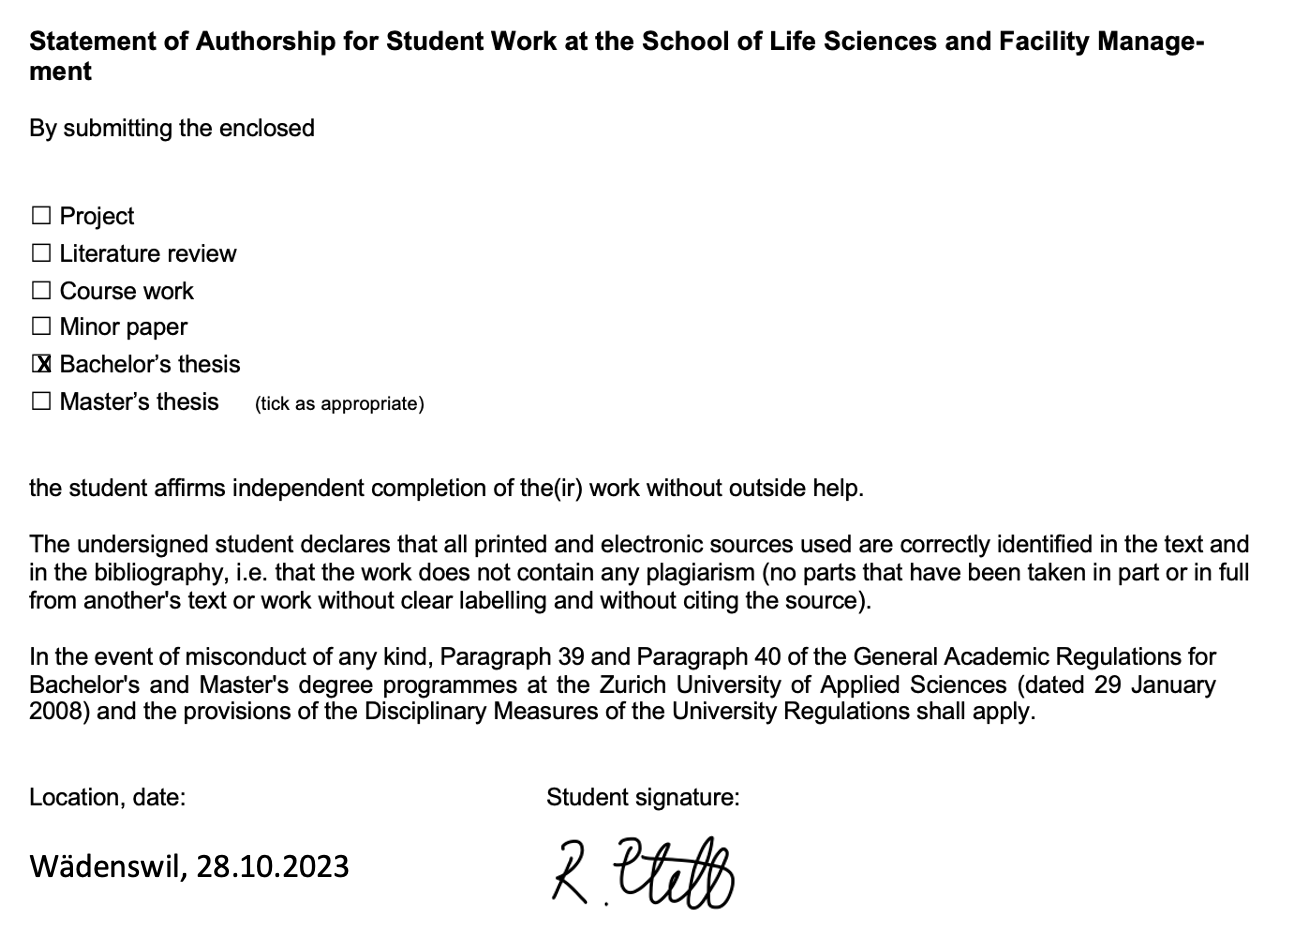
\includegraphics[width=1\textwidth,height=\textheight]{text/annex_files/plagiarism_declaration.png}{]}
\normalcolor \newpage

\hypertarget{sec-annex_ii}{%
\section*{\texorpdfstring{\textsc{II} Plagiarism
declaration}{ Plagiarism declaration}}\label{sec-annex_ii}}

\markright{\textsc{II} Plagiarism declaration}



\end{document}
